\documentclass[dvipdfmx,a4j,10pt, twocolumn]{jsarticle}
\input{packages.tex}
%--- Bibliography settings
\usepackage[backend=biber,style=numeric]{biblatex}
\addbibresource{refs.bib}
%-------------------------

\usepackage[margin=10mm]{geometry}
\pagestyle{empty} % ページ番号を消す
\begin{document}
\begin{titlepage}
    \begin{center}

        {\Large 提出日: \today}

        

        \vspace{40truept}

        

        \vspace*{180truept}

        {\Huge 研究プロジェクト課題} 
        \vspace{10truept}

        {\Huge }
        \vspace{160truept}


        {\Large 学籍番号: 23B30575}
        \vspace{10truept}

        \vspace{10truept}
        {\Large 氏名: 鳥光俊佑} 
        \vspace{10truept}

        {\Large }  

    \end{center}
\end{titlepage}
\newpage 

\title{Video Super-Resolution With Convolutional Neural Networks\cite{7444187} のまとめ}
\author{鳥光 俊佑}
\maketitle



\setlength{\columnseprule}{0.4pt} % 列の区切り線の太さを設定





\section*{なんのための研究か}

UHDテレビの普及に伴い, 低画質映像から
高画質映像へ変換する超解像アルゴリズム(SRアルゴリズム)が求められている。

この研究は, CNNを映像の超解像へ
応用し, 静止画での事前学習と時間的に連続するフレームの
統合により, 従来より高速かつ高画質な超解像を実現する研究である。

\section*{従来のアプローチとその問題点}

\subsection*{モデルベースのアプローチ}
モデルベースのアプローチとして, 
事前分布をもちいたベイズ推定に基づく手法が提案されている。

この手法は後述するCNNベースの手法と比較して計算コストが高いという問題がある。

\subsection*{学習ベースのアプローチ}

学習ベースのアプローチとして
辞書学習に基づく手法が紹介されている。
この手法では, 低解像度画像と高解像度画像のパッチペアから辞書を学習し, 
辞書の元の線型結合として画像を再構成する。

この手法では, 画像の再構成もパッチごとに行うため, 計算コストが高いという問題がある。

\subsection*{単一画像にCNNを用いたアプローチ}

単一画像の超解像にCNNを用いる手法(SR CNN)も提案されている。CNNベースの手法では, 
画像を超解像する処理は順伝播しょりによって行われるため, ベイズのような方法と異なり反復計算を必要としない。

しかし, この手法では映像の時間次元の情報を活用できないという問題がある。


\section*{この論文でのアプローチ}

この論文では, SR CNNを拡張し連続する複数のフレームを入力とするCNN(VSRnet)を提案している。

また, 隣接するフレーム間の影響によるフレーム間の位置のずれを削減する手法として
Adaptive Motion Compensation(AMC)を提案している。

さらに, 静止画を使用してモデルを事前学習することで
映像データが不足していても高精度な超解像を実現する手法についても述べている。


\section*{この論文で用いられるアプローチの新規性}

VSRnetの新規性は以下の3点である。

\begin{itemize}
    \item 従来のCNNベースの手法は単一画像を対象としていたが, VSRnetでは映像の時間的連続性を考慮するため連続する複数フレームを入力とするCNNを提案している。
    \item Motion Compensationについて, 従来のオプティカルフローに基づく手法とは異なり隣接フレームの影響を考慮するAMC (Adaptive Motion Compensation) を提案している。
    \item 静止画上でSRアーキテクチャを事前学習し, その得られたパラメータで映像用SRアーキテクチャの学習を初期化する手法を提案している。
\end{itemize}

\section*{この論文により出来るようになったこと}

VSRnetは, 従来の最高制度である手法(ベイズ推定, SRCNN)を
上回るPSNR, SSIMを達成していることが実験により確認された。

また, GPUのサポートによって, 従来のベイズ法の66倍ほどの高速化を実現した。

出力映像の視覚的品質についても, ベイズ推定による手法と比較してリンギングアーティファクトが少なく,
高精細な映像を生成できることが確認された。

\section*{鍵となる式や図}

\subsection*{隣接フレームの結合方式の比較}

論文中のFig. 2では, 映像用SRアーキテクチャにおける連続時間のフレーム結合方式の比較が示されている。

\begin{figure}[H]
    \centering
    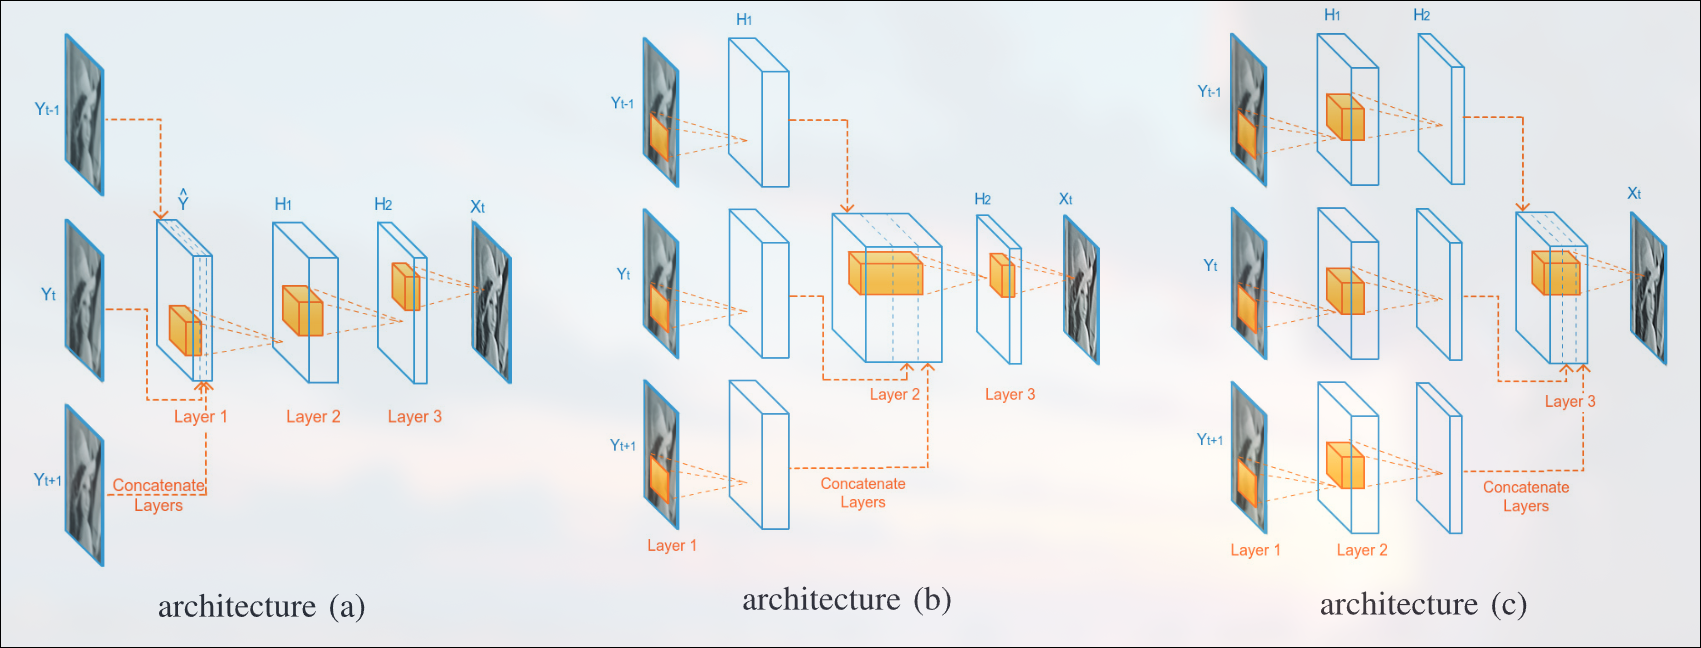
\includegraphics[width=9cm]{1.png}
    \caption{映像用SRアーキテクチャにおけるフレームの結合方式の比較}
    \label{fig:frame_comb}
\end{figure}

映像用SRアーキテクチャは3つの層からなり, 図\ref{fig:frame_comb}
で示されている(a), (b), (c)のアーキテクチャはそれぞれ:
\begin{itemize}
    \item (a) 入力層でフレームを結合
    \item (b) 中間層で各フレームを独立に処理した後, 結合する方式
    \item (c) 各フレームを独立に処理し, 最終層で結合する方式
\end{itemize}

となっている。どの方式の性能を似通ってはいるもの、実験により(b)の方式が最高のPNSRを達成することが確認されている。
また, 論文中のFig. 6では
図\ref{fig:frame_comb2}のように(b)の方式が学習時間と性能のバランスで最も優れていることが示されている。

\begin{figure}[H]
    \centering
    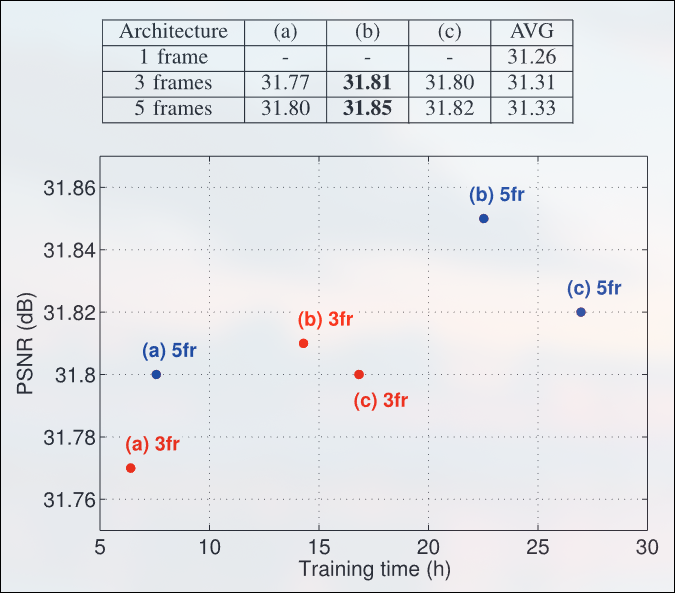
\includegraphics[width=9cm]{2.png}
    \caption{各方式の学習時間とPSNR}
    \label{fig:frame_comb2}
\end{figure}

\subsection*{AMCの定義式}

論文中の式(6), (7)ではAMCの定義が示されている。

\begin{align*}
y_{t-T}^{amc}(i,j) &= (1-r(i,j))y_t(i,j) + r(i,j)y_{t-T}^{MC}(i,j) \tag{6}\\ 
r(i,j) &= \exp (-ke(i,j)) \tag{7}
\end{align*}


各変数の意味は以下の通りである。
\begin{itemize}
    \item $y_{t-T}^{amc}(i,j)$: AMC後のフレーム$t-T$の値
    \item $y_t(i,j)$: 現在のフレーム$t$の値
    \item $y_{t-T}^{MC}(i,j)$: Motion Compensationを行った後のフレーム$t-T$の値
    \item $r(i,j)$: ピクセル$(i,j)$における重み（隣接フレームの信頼度と見做せる）
    \item $e(i,j)$: ピクセル$(i,j)$におけるMotion Compensationの誤差
    \item $k$: 定数
\end{itemize}

AMCの定義式から, $r(i,j)$が小さいほど, 
隣接フレームの信頼性が低いと判断され, 現在のフレームの値で埋めようとすることがわかる。

AMCがない場合は, 信頼度の低い隣接フレームの情報も使用してしまうため, 
出力画像にアーティファクトが発生しやすくなる。AMCを用いることで,
隣接フレームの信頼性に応じて情報を取捨選択できるため, 高精度な超解像が可能になると考えられる。

\subsection*{事前学習させた重みの転移}

事前学習モデルでは, 単一の画像を入力とするが, 映像用SRアーキテクチャでは
複数のフレームを入力とする。そのため, 入力チャネル数が異なる事前学習モデル
の重みをそのまま利用することはできない。

論文中の式(5)では, 重みを転移させる具体的な数式が示されている。

\begin{align*}
w_v(m, n, t- 1, c) = w_v(m, n, t, c) &= w_v(m, n, t+ 1, c)\\
&= \frac{1}{3}w(m, n, t, c) \tag{5}
\end{align*}

各変数の意味は以下の通りである。
\begin{itemize}
    \item $w_v(m,n,t,c)$: 映像用SRアーキテクチャの重み
    \item $w(m,n,t,c)$: 事前学習モデルの重み
\end{itemize}


論文では, 以下の仮定を置いている:
映像用SRアーキテクチャで3つの等価なフレームを入力とした場合, 
その出力は事前学習モデルに単一のフレームを入力した場合と同じになるべきである。

この仮定に基づき計算していくことで, 式(5)のような重みの転移方法が導出される。

論文では, (a), (b), (c)の3つのアーキテクチャが提案されているが, フレーム結合のタイミングによって
重みを拡張する層が異なることに注意が必要である。

\section*{実験と評価方法}

\subsection*{データセット}
Myanmar video sequence(3840x2160から960x540にダウンサンプリングしたもの)とVideoset4
データセットが使用された。

\subsection*{比較対象}
Bicubic, ScSR, A+, SRCNN, ANN, ベイズ推定法, Video Enhencer, VSRnet(提案手法)が比較対象として使用された。
\subsection*{評価方法}
PSNR, SSIMが評価指標として使用された。また, 実行時間による評価も行われた。


\section*{この論文の手法の課題}

\subsection*{オプティカルフローアルゴリズムへの依存}

AMCの定義式はオプティカルフローアルゴリズムによって計算される
Motion Compensationに依存している。オプティカルフローアルゴリズムによる
推定が難しい領域では, AMCの効果も期待できない可能性がある。

\subsection*{ReLU関数の特性}

ReLU関数の副作用として, いくつかのフィルタが機能しなくなることが観察された。
更新ステップの間に大きな重みの更新が生じた際, 
ReLU関数の特性により, いくつかのニューロンの勾配が0になり続けてしまうことが原因とされている。

\section*{次に読むべき論文}

オプティカルフローアルゴリズムへ依存しない, Motion Compensationの手法について述べた論文と
して次の論文を挙げる。

Real-Time Video Super-Resolution with Spatio-Temporal Networks and Motion Compensation \cite{8099787}

この論文では, 
Spatial Transformer Networkを用いたMotion Compensationの手法が述べられている。


\printbibliography[title=参考文献] % 参考文献の出力. 参考文献が不要ならばコメントアウトする.
\end{document}
